\documentclass{standalone}
\usepackage{tikz}

\begin{document}

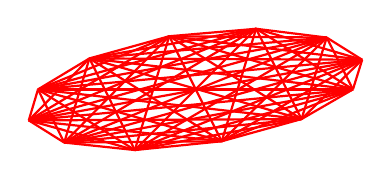
\begin{tikzpicture}[scale=2]
    % Define the vertices of the polyhedron
    \def\n{12} % Number of vertices
    \def\r{1}  % Radius of the circumscribed sphere
    \def\phi{0.5513} % Golden ratio angle
    
    \foreach \i in {1,...,\n} {
        \pgfmathsetmacro{\theta}{\i * 360 / \n}
        \pgfmathsetmacro{\phi}{\phi * cos(\theta)}
        \pgfmathsetmacro{\x}{\r * sin(\theta) * cos(\phi)}
        \pgfmathsetmacro{\y}{\r * sin(\theta) * sin(\phi)}
        \pgfmathsetmacro{\z}{\r * cos(\theta)}
        \coordinate (v\i) at (\x,\y,\z);
    }
    
    % Draw the edges of the polyhedron
    \foreach \i in {1,...,\n} {
        \foreach \j in {\i,...,\n} {
            \draw[red, thick] (v\i) -- (v\j);
        }
    }
    
    % Optionally, draw the faces if needed
    % \foreach \i in {1,...,\n} {
    %     \foreach \j in {\i,...,\n} {
    %         \draw[blue!50!cyan, fill=blue!20] (v\i) -- (v\j) -- (v\k) -- cycle;
    %     }
    % }
    
\end{tikzpicture}

\end{document}